%%%%%%%%%%%%%%%%%%%%%%%%%%%%%%%%%%%%%%%%%
% Beamer Presentation
% LaTeX Template
% Version 1.0 (10/11/12)
%
% This template has been downloaded from:
% http://www.LaTeXTemplates.com
%
% License:
% CC BY-NC-SA 3.0 (http://creativecommons.org/licenses/by-nc-sa/3.0/)
%
%%%%%%%%%%%%%%%%%%%%%%%%%%%%%%%%%%%%%%%%%

%----------------------------------------------------------------------------------------
%	PACKAGES AND THEMES
%----------------------------------------------------------------------------------------

\documentclass{beamer}

\mode<presentation> {

% The Beamer class comes with a number of default slide themes
% which change the colors and layouts of slides. Below this is a list
% of all the themes, uncomment each in turn to see what they look like.

%\usetheme{default}
%\usetheme{AnnArbor}
%\usetheme{Antibes}
%\usetheme{Bergen}
%\usetheme{Berkeley}
%\usetheme{Berlin}
%\usetheme{Boadilla}
%\usetheme{CambridgeUS}
%\usetheme{Copenhagen}
%\usetheme{Darmstadt}
%\usetheme{Dresden}
%\usetheme{Frankfurt}
%\usetheme{Goettingen}
%\usetheme{Hannover}
%\usetheme{Ilmenau}
%\usetheme{JuanLesPins}
%\usetheme{Luebeck}
\usetheme{Madrid}
%\usetheme{Malmoe}
%\usetheme{Marburg}
%\usetheme{Montpellier}
%\usetheme{PaloAlto}
%\usetheme{Pittsburgh}
%\usetheme{Rochester}
%\usetheme{Singapore}
%\usetheme{Szeged}
%\usetheme{Warsaw}

% As well as themes, the Beamer class has a number of color themes
% for any slide theme. Uncomment each of these in turn to see how it
% changes the colors of your current slide theme.

%\usecolortheme{albatross}
%\usecolortheme{beaver}
%\usecolortheme{beetle}
%\usecolortheme{crane}
%\usecolortheme{dolphin}
%\usecolortheme{dove}
%\usecolortheme{fly}
%\usecolortheme{lily}
%\usecolortheme{orchid}
%\usecolortheme{rose}
%\usecolortheme{seagull}
%\usecolortheme{seahorse}
%\usecolortheme{whale}
%\usecolortheme{wolverine}

%\setbeamertemplate{footline} % To remove the footer line in all slides uncomment this line
%\setbeamertemplate{footline}[page number] % To replace the footer line in all slides with a simple slide count uncomment this line

%\setbeamertemplate{navigation symbols}{} % To remove the navigation symbols from the bottom of all slides uncomment this line
}

\usepackage[brazilian,english]{babel}
\usepackage[utf8]{inputenc}
\usepackage{aeguill}

\usepackage{graphicx} % Allows including images
\usepackage{booktabs} % Allows the use of \toprule, \midrule and \bottomrule in tables



%\usepackage[utf8]{inputenc}
%\usepackage[portuges]{babel}
%\usepackage[brazilian]{babel}
%\usepackage[utf8]{inputenc}
%\usepackage[T1]{fontenc}

%----------------------------------------------------------------------------------------
%	TITLE PAGE
%----------------------------------------------------------------------------------------

\title[DELET-UFRGS]{Abordagem Fuzzy para identifica\c{c}\~ao de Partos Prematuros e N\~ao-Prematuros} % The short title appears at the bottom of every slide, the full title is only on the title page

\author{Tondin B., Chedid R. e Balbinot A.} % Your name
\institute[UFRGS] % Your institution as it will appear on the bottom of every slide, may be shorthand to save space
{
Universidade Federal do Rio Grande do Sul \\ % Your institution for the title page
\medskip
\textit{btondin@hcpa.edu.br, raissan@gmail.com} % Your email address
}
\date{ 22 de Maio de 2017} % Date, can be changed to a custom date

\begin{document}

\begin{frame}
\titlepage % Print the title page as the first slide
\end{frame}

\begin{frame}
\frametitle{Conte\'udo} % Table of contents slide, comment this block out to remove it
\tableofcontents % Throughout your presentation, if you choose to use \section{} and \subsection{} commands, these will automatically be printed on this slide as an overview of your presentation
\end{frame}

%----------------------------------------------------------------------------------------
%	PRESENTATION SLIDES
%----------------------------------------------------------------------------------------]

%------------------------------------------------
\section{Objetivos} % Sections can be created in order to organize your presentation into discrete blocks, all sections and subsections are automatically printed in the table of contents as an overview of the talk
%------------------------------------------------

%------------------------------------------------
\section{Introdu\c{c}\~ao} 

%\subsection{O parto prematuro } % A subsection can be created just before a set of slides with a common theme to further break down your presentation into chunks

%\subsection{Tocodinamometria }

%-------------------------

%------------------------------------------------
\section{A base de dados} 
%-------------------------



%------------------------------------------------
\section{Metodologia} 
%-------------------------

%------------------------------------------------
\section{Resultados} 
%-------------------------

%------------------------------------------------
\section{Conclus\~ao} 
%-------------------------



\begin{frame}
\frametitle{Objetivos}

Avaliar a possibilidade de detecção de partos prematuros ou não-prematuros utilizando lógica {\em fuzzy} em sinais de eletromiografia uterina [eletrohisterograma (EHG)] do abdômen de mulheres em gestação.

\begin{itemize}
	\item Os autores não encontraram, até o presente momento, outros trabalhos utilizando lógica {\em fuzzy} em sinais de EHG;
	\item permitir a comparação futura com outros métodos de classificação.
\end{itemize}

\end{frame}

%------------------------------------------------

\begin{frame}
	\frametitle{Introdu\c{c}\~ao: o parto prematuro}	
	
	\begin{itemize}
		\item Gravidez é um processo fisiológico que envolve mudanças anatômicas, psicológicas e emocionais, resultado de um incremento hormonal que permite cumprir as demandas metabólicas do feto e da mãe \cite{p1};
		\item apesar de ser um processo natural, a gravidez pode acarretar diversos problemas de saúde que, nas formas mais graves, constituem em uma proporção significante da mortandade de mulheres jovens \cite{p2};
		\item uma das maiores causas desta mortandade é o parto prematuro \cite{p2}.
	\end{itemize}
	
\end{frame}
 
%------------------------------------------------

\begin{frame}
	\frametitle{Introdu\c{c}\~ao: tocodinamometria}	
	
	É a técnica mais utilizada na atualidade para avaliar a força, duração e frequência de contrações uterinas. É um sensor de pressão que apresenta as contrações em um gráfico tempo X pressão. Possui as seguintes desvantagens:
	
	\begin{itemize}
		
		\item interpretação varia de paciente para paciente e de operador para operador  \cite{ref-bernardes};
		
		\item eventualmente, há mudança (para cima ou para baixo) na linha de base do sinal, o que dificulta a interpretação. Isso é conhecido como {\em baseline errante} \cite{ref-marques}.
		
	\end{itemize}
	
\end{frame}

%------------------------------------------------


\begin{frame}
	\frametitle{Introdu\c{c}\~ao: tocodinamometria}	

 \begin{figure}[H]
 	\caption{\label{toco} Contrações uterinas medidas com tocodinamometria.}
 	\begin{center}
 		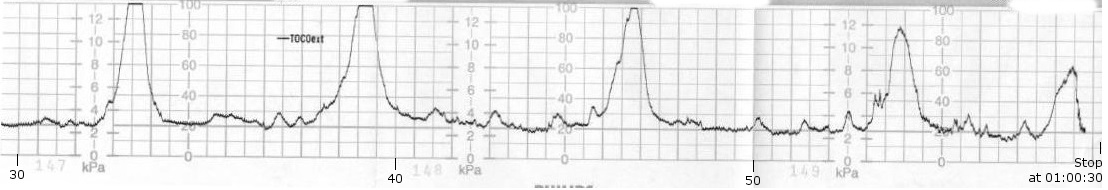
\includegraphics[scale=0.40]{imagens/toco.jpg} 		
 	\end{center}
 	%\legend{\cite{ref-islddatabase}}
 \end{figure}
 
 Fonte: \cite{ref-islddatabase}
 
 
\end{frame}

%------------------------------------------------

\begin{frame}
	\frametitle{Introdu\c{c}\~ao: eletromiografia uterina}	
	
	Também chamada de EHG (eletrohisterografia), avalia a atividade elétrica uterina no domínio do tempo, através de eletrodos de superfície fixados no abdômen da gestante. Esses sinais elétricos são os comandos para que o útero se contraia. 
	
	\begin{itemize}
		
		\item O nível de atividade aumenta conforme se aproxima o dia do parto e, nos últimos 3 ou 4 dias há um salto considerável na mesma \cite{ref-lucovnik};
		
		\item antes de permitir uma análise apropriada, o sinal obtido, na sua forma bruta, necessita de um pré processamento. Podem ser utilizados, filtros, removedores de ruído e detecção automática de contrações.
		
	\end{itemize}
	
\end{frame}

%------------------------------------------------


\begin{frame}
	\frametitle{Introdu\c{c}\~ao: tocodinamometria}	
	
	\begin{figure}[H]
		\caption{\label{barrigao} Posicionamento do tocodonamômetro e dos eletrodos e EHG.}
		\begin{center}
			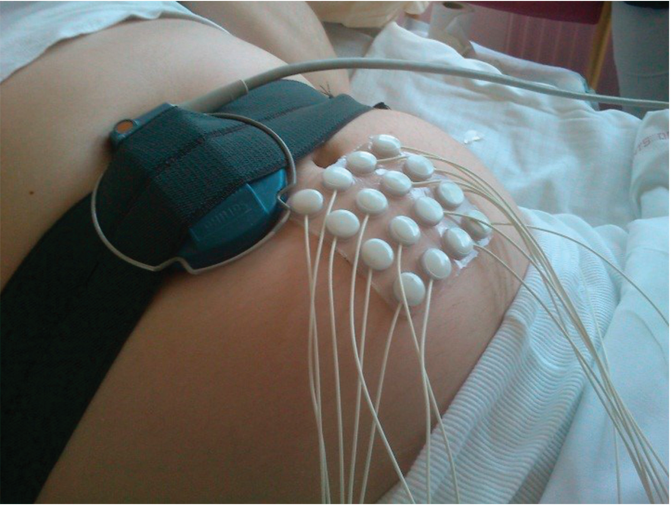
\includegraphics[scale=0.35]{imagens/barrigao.png} 		
		\end{center}
		%\legend{\cite{ref-islddatabase}}
	\end{figure}
	
	Fonte: \cite{ref-islddatabase}
	
\end{frame}

%------------------------------------------------

\begin{frame}
	\frametitle{A base de dados}	
	
	\begin{itemize}
	
		\item As aquisições utilizadas neste trabalhos foram feitas na Eslovênia entre 1997 e 2005 utilizando um equipamento 4 eletrodos de superfície de forma bipolar, resultando em 3 canais;
		
		\item São 300 medições feitas durante {\em check-ups} regulares, onde 38 são de nascimentos prematuros e 262 de nascimentos não-prematuros;
		
		\item a frequência de amostragem foi de 20Hz com uma resolução de 16bits \cite{Kavšek}.
	
	\end{itemize}
	
\end{frame}

%------------------------------------------------

\begin{frame}
	\frametitle{Metodologia: pré-processamento}	
	
	O pré-processamento do sinal foi feito da seguinte forma: 
	
	\begin{itemize}
		
		\item conforme \cite{ref-lucovnik}, a faixa de frequência onde se concentra a maior parte do sinal relevante, e se rejeita a maior parte dos artefatos indesejados é de 0.34 a 1Hz. Portando o sinal foi filtrado utilizando um filtro passa faixa Butterworth de oitava ordem nesta faixa de frequência;
		
		\item o ruído foi removido utilizando a transformada de Wavelet, onde a função escolhida para a mesma foi a Daubechies4 com nível 10 e limiar suave universal;
		
		\item a segmentação do sinal foi feita a mão pois permitiu fazer uma separação dos artefatos de movimento oriundos da atividade do feto.
		
	\end{itemize}
	
\end{frame}

%------------------------------------------------


\begin{frame}
	\frametitle{Metodologia: extração de características}	
	
	Características avaliadas para as contrações: 
	
	\begin{itemize}
		
		\item RMS (máximo, mínimo e médio);
		
		\item variância (máxima, mínima e média);
		
		\item frequência de pico (máxima, mínima e média);
		
		\item duração média;
		
		\item frequência média entre contrações;
		
		\item intervalo médio entre contrações.
		
		
		
	\end{itemize}
	
\end{frame}

%------------------------------------------------












%------------------------------------------------

\begin{frame}
	\frametitle{Resultados: pré-processamento}	
	
	\begin{figure}[H]
		\caption{\label{sinais} Resultado do pré-processamento.}
		\begin{center}
			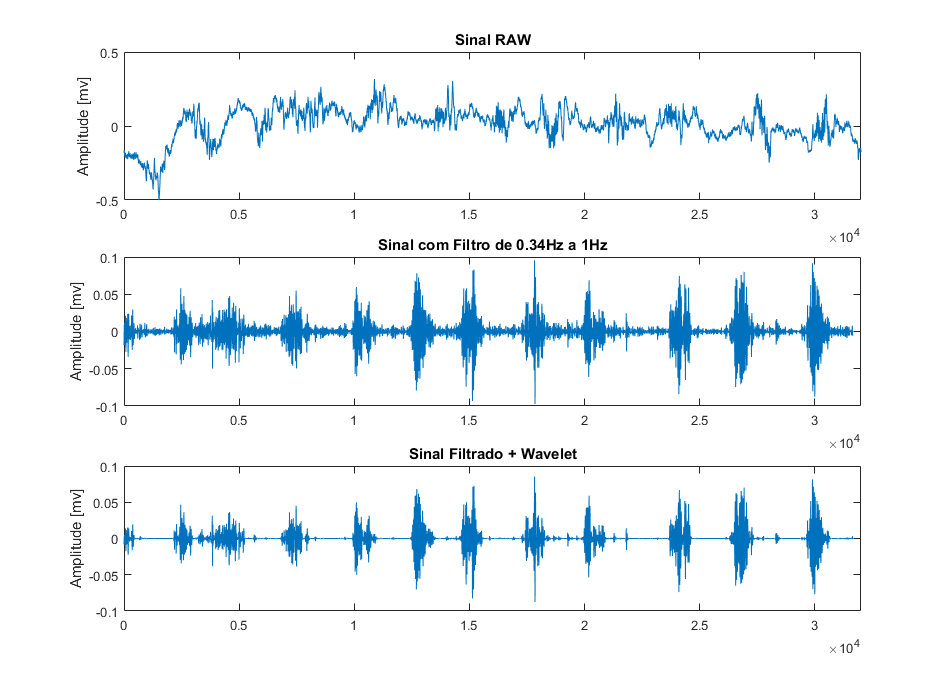
\includegraphics[scale=0.33]{imagens/sinais.png} 		
		\end{center}
		%\legend{\cite{ref-islddatabase}}
	\end{figure}
	
	Fonte: [Autores]
	
\end{frame}

%------------------------------------------------

\begin{frame}
\frametitle{Bullet Points}
\begin{itemize}
\item Lorem ipsum dolor sit amet, consectetur adipiscing elit
\item Aliquam blandit faucibus nisi, sit amet dapibus enim tempus eu
\item Nulla commodo, erat quis gravida posuere, elit lacus lobortis est, quis porttitor odio mauris at libero
\item Nam cursus est eget velit posuere pellentesque
\item Vestibulum faucibus velit a augue condimentum quis convallis nulla gravida
\end{itemize}
\end{frame}

%------------------------------------------------

\begin{frame}
\frametitle{Blocks of Highlighted Text}
\begin{block}{Block 1}
Lorem ipsum dolor sit amet, consectetur adipiscing elit. Integer lectus nisl, ultricies in feugiat rutrum, porttitor sit amet augue. Aliquam ut tortor mauris. Sed volutpat ante purus, quis accumsan dolor.
\end{block}

\begin{block}{Block 2}
Pellentesque sed tellus purus. Class aptent taciti sociosqu ad litora torquent per conubia nostra, per inceptos himenaeos. Vestibulum quis magna at risus dictum tempor eu vitae velit.
\end{block}

\begin{block}{Block 3}
Suspendisse tincidunt sagittis gravida. Curabitur condimentum, enim sed venenatis rutrum, ipsum neque consectetur orci, sed blandit justo nisi ac lacus.
\end{block}
\end{frame}

%------------------------------------------------

\begin{frame}
\frametitle{Multiple Columns}
\begin{columns}[c] % The "c" option specifies centered vertical alignment while the "t" option is used for top vertical alignment

\column{.45\textwidth} % Left column and width
\textbf{Heading}
\begin{enumerate}
\item Statement
\item Explanation
\item Example
\end{enumerate}

\column{.5\textwidth} % Right column and width
Lorem ipsum dolor sit amet, consectetur adipiscing elit. Integer lectus nisl, ultricies in feugiat rutrum, porttitor sit amet augue. Aliquam ut tortor mauris. Sed volutpat ante purus, quis accumsan dolor.

\end{columns}
\end{frame}

%------------------------------------------------
\section{Second Section}
%------------------------------------------------

\begin{frame}
\frametitle{Table}
\begin{table}
\begin{tabular}{l l l}
\toprule
\textbf{Treatments} & \textbf{Response 1} & \textbf{Response 2}\\
\midrule
Treatment 1 & 0.0003262 & 0.562 \\
Treatment 2 & 0.0015681 & 0.910 \\
Treatment 3 & 0.0009271 & 0.296 \\
\bottomrule
\end{tabular}
\caption{Table caption}
\end{table}
\end{frame}

%------------------------------------------------

\begin{frame}
\frametitle{Theorem}
\begin{theorem}[Mass--energy equivalence]
$E = mc^2$
\end{theorem}
\end{frame}

%------------------------------------------------

\begin{frame}[fragile] % Need to use the fragile option when verbatim is used in the slide
\frametitle{Verbatim}
\begin{example}[Theorem Slide Code]
\begin{verbatim}
\begin{frame}
\frametitle{Theorem}
\begin{theorem}[Mass--energy equivalence]
$E = mc^2$
\end{theorem}
\end{frame}\end{verbatim}
\end{example}
\end{frame}

%------------------------------------------------

\begin{frame}
\frametitle{Figure}
Uncomment the code on this slide to include your own image from the same directory as the template .TeX file.
%\begin{figure}
%\includegraphics[width=0.8\linewidth]{test}
%\end{figure}
\end{frame}

%------------------------------------------------

\begin{frame}[fragile] % Need to use the fragile option when verbatim is used in the slide
\frametitle{Citation}
An example of the \verb|\cite| command to cite within the presentation:\\~

This statement requires citation \cite{p1}.
\end{frame}

%------------------------------------------------

\begin{frame}
\frametitle{References}
\footnotesize{
\begin{thebibliography}{99} % Beamer does not support BibTeX so references must be inserted manually as below
\bibitem[Weissgerber, 2006]{p1} T.L. Weissgerber, L.A. Wolfe (2006)
\newblock Physiological adaptation in early human pregnancy: adaptation to balance maternal-fetal demands.
\newblock \emph{Appl. Physiol. Nutr. Metab} 31, 1 -- 11.

\bibitem[Alkema L., 2016]{p2} Alkema L. {\em et al} (2016)
\newblock Global, regional, and national levels and trends in maternal mortality between 1990 and 2015, with scenario-based projections to 2030: a systematic analysis by the UN Maternal Mortality Estimation Inter-Agency Group.
\newblock \emph{Lancet} 387, 462 -- 74.

\bibitem[Bernardes J., 1997]{ref-bernardes} J. Bernardes, A. Costa-Pereira, D. Ayres-de-Campos, H. Van Geijn, and L. Pereira-Leite. (1997)
\newblock Evaluation of interobserver agreement of Cardiotocograms
\newblock \emph{International Journal of Gynaecology \& Obstetrics.} 57, 33 -- 37.

\bibitem[Marques J.A., 2013]{ref-marques} J. A. Marques, P. C. Cortez, J. P. Madeiro, and F. S. Schlindwein (2013)
\newblock Computerized Cardiotocography analysis system based on Hilbert Transform
\newblock \emph{Expert System with Applications.} 40, 7159 -- 7658.
\end{thebibliography}
}
\end{frame}

%------------------------------------------------

\begin{frame}
	\frametitle{References}
	\footnotesize{
		\begin{thebibliography}{99} % Beamer does not support BibTeX so references must be inserted manually as below
						
			\bibitem[Lucovnik M., 2011]{ref-lucovnik} Lucovnik M., Maner W.L., Chambliss L.R. {\em et al} (2011)
			\newblock Noninvasive uterine electromyography for prediction of preterm delivery.
			\newblock \emph{American journal of obstetrics and gynecology} 204(3),  228.e1 -- 10.
			
			\bibitem[Alexandersson A. 2015]{ref-islddatabase} Alexandersson A., Steingrimsdottir T., Terrien j. {\em et al} (2015)
			\newblock The Icelandic 16-electrode electrohysterogram database.
			\newblock \emph{Sci. Data}.
			
			\bibitem[Kavšek, G. 2001]{Kavšek} Kavšek, G. (2001)
			\newblock Electromyographic activity of the uterus in threatened preterm delivery.
			\newblock \emph{MsC thesis}.
			
			
		\end{thebibliography}
	}
\end{frame}

%------------------------------------------------

\begin{frame}
\Huge{\centerline{Fim}}
\end{frame}

%----------------------------------------------------------------------------------------

\end{document} 